\documentclass{article}
% 默认字体大小是
% Formatting
\usepackage[utf8]{inputenc}
\usepackage[margin=1in]{geometry}
\usepackage[titletoc,title]{appendix}

\usepackage{amsmath,amsfonts,amssymb,mathtools}
\usepackage{graphicx,float}
\usepackage{booktabs}
\usepackage[ruled,vlined]{algorithm2e}
\usepackage{algorithmic}
\usepackage{biblatex}
\usepackage{cleveref}
\usepackage{indentfirst}
\setlength{\parindent}{2em}

\addbibresource{references.bib}

\title{PRML Spring 2026 Homework 1}
\author{Yifan Ding \\
        \small Code: \url{https://github.com/douhenhuidyf/PRML-Spring-2026/tree/main/hw1} \\
        \small Email: 23373493@buaa.edu.cn}
\date{March 24, 2026}

\begin{document}
\maketitle

\begin{abstract}
Regression analysis is a fundamental statistical technique used to model and analyze the relationship between a dependent variable and one or more independent variables.
The core challenge of regression lies in finding a robust mapping from input features to continuous output values with high accuracy and generalization ability.,
where the choice of model and optimization algorithm directly impacts its performance.

In this paper, we explore the performance of different regression models and optimization algorithms on a given dataset.
We evaluate linear regression using least squares, gradient descent, and Newton's method, and find that it does not fit the data well due to the nonlinear relationship between the input features and the output values. 
We then apply polynomial regression with varying degrees and observe that it provides a better fit to the data, but there is a risk of overfitting as the degree increases and cost more computational resources. 
Finally, we implement kernel regression using a Gaussian kernel and find that it achieves the best results, although its performance is highly sensitive to the choice of bandwidth parameter. 

Overall, our findings highlight the importance of selecting appropriate models and optimization algorithms based on the characteristics of the data and the underlying relationships between variables.
\end{abstract}


\section{Introduction}
\subsection{Problem Statement}
Given a set of 2D data: Data4Regression, where the first sheet is training data and the second sheet is testing data.
\begin{enumerate}
    \item Use least squares, gradient descent (GD), and Newton's method to perform linear fitting on the data,
     and observe their training and testing errors.
    \item If you find that the linear model does not fit well (the data is actually nonlinear,
     so it is normal that the experimental results of the previous question are not good),
      can you find a more suitable model to fit the given data?
    Please give the reason for choosing the model, specific experimental results, and analysis of the results.
\end{enumerate}

\subsection{Problem Analysis}
Firstly, let's take a look at the distribution of the data.
\begin{figure}[H]
    \centering
    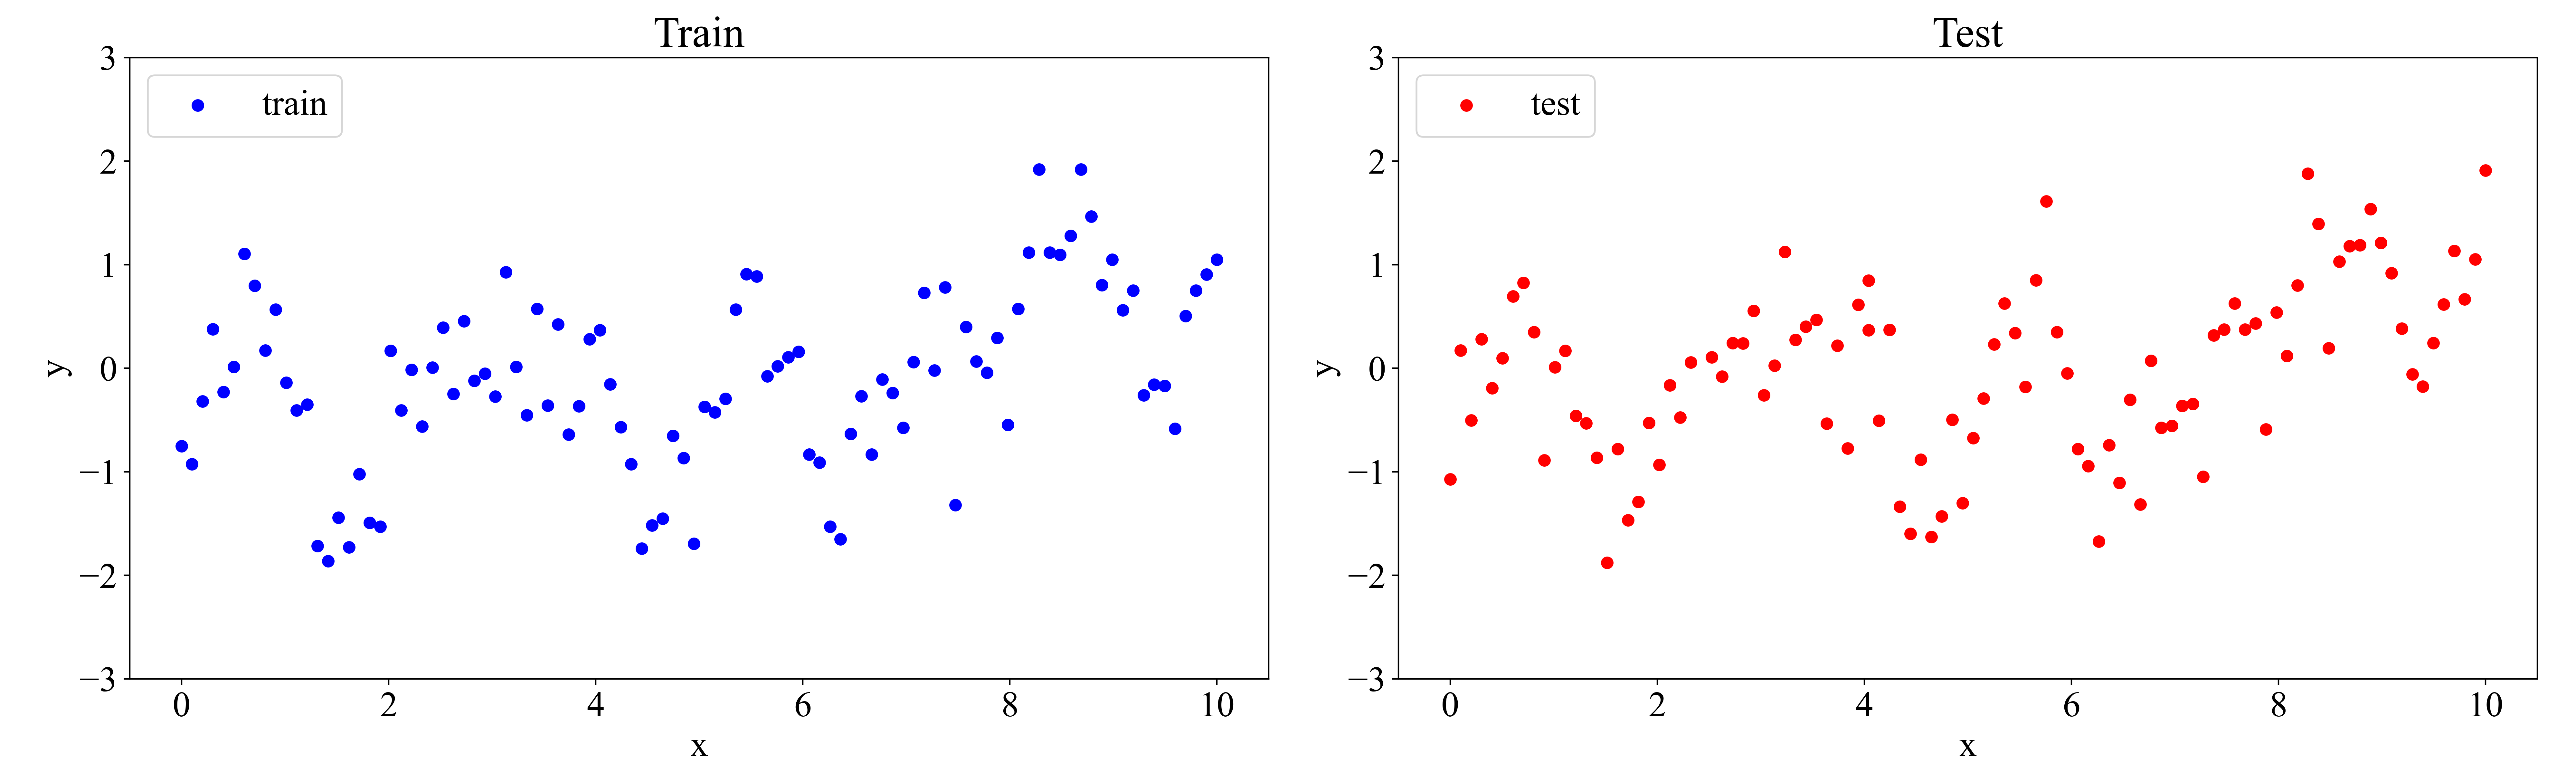
\includegraphics[width=0.8\linewidth]{figure/data_distribution.png}
    \caption{Distribution of given training and testing data.}
    \label{fig:distrubution}
\end{figure}
As shown in \Cref{fig:distrubution}, the data is not linearly distributed, so we can expect that the linear regression model will not work well.
In such cases, we should consider using a nonlinear regression model to capture the underlying patterns in the data.

Here are some potential nonlinear regression models that we can consider:
\begin{itemize}
    \item Polynomial Regression: This model fits a polynomial function to the data, allowing for more flexibility in capturing nonlinear relationships.
    \item Kernel Regression: This model uses a kernel function to measure the similarity between data points, allowing for nonlinear relationships to be captured without explicitly defining a polynomial function.
    \item Neural Networks(NNs): Supported by Universal Approximation Theorem, neural networks with multiple layers of interconnected nodes can learn complex nonlinear relationships between the input features and the output values.
        Training a neural network can be computationally expensive and may require a large amount of data.
\end{itemize}

Due to the limited amount of data(100 for train and 100 for test), we will focus on polynomial regression and kernel regression in our experiments.

\subsection{Structure of the Paper}
The rest of this paper is organized as follows: In \Cref{sec:methodology}, we will discuss the metrics used to evaluate the performance of different models and optimization algorithms, and introduce the baseline model (linear regression) and the nonlinear regression models (polynomial regression and kernel regression) that we will be using in our experiments.
In \Cref{sec:experiments}, we will present the experimental results of applying these models to the given data, and analyze the results. Finally, we will conclude the paper in \Cref{sec:conclusions}.

\section{Methodology}
\label{sec:methodology}
\subsection{Metrics}
\label{sec:metrics}
To evaluate the performance of different models and algorithms, we can use two common metrics: root mean squared error (RMSE) and coefficient of determination ($R^2$).
The RMSE is defined as:
\begin{equation}
    RMSE = \sqrt{\frac{1}{n} \sum_{i=1}^{n} (y_i - \hat{y}_i)^2},
\end{equation}
where $y_i$ is the true value and $\hat{y}_i$ is the predicted value.
The RMSE measures the average squared difference between the true values and the predicted values,
and a lower RMSE indicates a better fit of the model to the data.

The coefficient of determination, denoted as $R^2$, is defined as:
\begin{equation}
    R^2 = 1 - \frac{\sum_{i=1}^{n} (y_i - \hat{y}_i)^2}{\sum_{i=1}^{n} (y_i - \bar{y})^2},
\end{equation}
where $\bar{y}$ is the mean of the true values. The $R^2$ value ranges from 0 to 1, where a value closer to 1
indicates that the model explains a larger proportion of the variance in the dependent variable.

\subsection{Baseline Model: Linear Regression}
Linear regression is a fundamental statistical method used to model the relationship between a dependent variable 
and one or more independent variables. The goal of linear regression is to find the best-fitting line (or hyperplane in higher dimensions) 
that minimizes the sum of squared differences between the observed values and the predicted values. 
The linear regression model can be expressed as:
\begin{equation}
    y = \beta_0 + \beta_1 x_1 + \beta_2 x_2 + \ldots + \beta_p x_p,
\end{equation}
where $y$ is the dependent variable, $x_1, x_2, \ldots, x_p$ are the independent variables, $\beta_0$ is the intercept,
 $\beta_1, \beta_2, \ldots, \beta_p$ are the coefficients.

Here we will discuss three optimal algorithms for fitting a linear regression model: least squares, gradient descent, and Newton's method.

\subsubsection{Least Squares}
The least squares method is a mathematical approach used to find the best-fitting line (or hyperplane in higher dimensions) in linear regression
by minimizing the sum of squared differences between the observed values and the predicted values.
Given a set of training data points $(x_i, y_i)$ for $i = 1, 2, \ldots, n$, the least squares method aims to find the coefficients $\beta_0, \beta_1, \ldots, \beta_p$ that minimize the cost function:
\begin{equation}
    J(\beta) = \sum_{i=1}^{n} (y_i - \hat{y}_i)^2,
\end{equation}
where $\hat{y}_i$ is the predicted value for the $i$-th data point, given by the linear model:
\begin{equation}
    \hat{y}_i = \beta_0 + \beta_1 x_{i1} + \beta_2 x_{i2} + \ldots + \beta_p x_{ip}.
\end{equation}
The least squares method can be solved analytically using the normal equation:
\begin{equation}
    \beta = (X^T X)^{-1} X^T y,
\end{equation}
where $X$ is the matrix of input features and $y$ is the vector of observed values.
This method provides a closed-form solution for the coefficients, making it computationally efficient for small datasets.
However, for larger datasets or when the number of features is high, it may be computationalally expensive due to the matrix inversion step,
which has a time complexity of $O(n^3)$, where $n$ is the number of data points.


\subsubsection{Gradient Descent}
Gradient descent(GD) is an optimization algorithm used to minimize the cost function in machine learning models,
 including linear regression.
Given a loss function $J(\theta)$, where $\theta$ represents the parameters of the model,
 the gradient descent algorithm iteratively updates the parameters in the direction of the negative gradient of the cost function with respect to the parameters. The update rule can be expressed as:
\begin{equation}
    \theta := \theta - \alpha \nabla J(\theta),
\end{equation}
where $\alpha$ is the learning rate, and $\nabla J(\theta)$ is the gradient of the cost function with respect to the parameters $\theta$.
The key idea behind gradient descent is to take small steps in the direction of the steepest descent of the cost function,
which helps to find the optimal parameters that minimize the cost function.

Several variants of gradient descent, such as stochastic gradient descent (SGD) and mini-batch gradient descent(MBGD),
have been developed to improve the efficiency of the algorithm.
But the misuse of learning rate can lead to divergence or slow convergence.
Techniques such as learning rate scheduling and momentum (e.g., Adam\cite{kingma2017adammethodstochasticoptimization}, AdamW\cite{loshchilov2019decoupledweightdecayregularization}) have been developed to address these issues and improve the performance of gradient descent.

In the context of linear regression, the gradient of the cost function with respect to the parameters can be computed as:
\begin{equation}
    \nabla J(\theta) = \nabla(\frac{1}{n} ||\mathbf{y} - \mathbf{X}\theta||^2) = -\frac{2}{n} X^T (\mathbf{y} - \mathbf{X}\theta),
\end{equation}
where $\mathbf{X}$ is the matrix of input features, $\mathbf{y}$ is the vector of observed values, and $\theta$ is the vector of parameters.
By iteratively updating the parameters using the gradient descent algorithm, we can find the optimal parameters that minimize the cost function and improve the fit of

\subsubsection{Newton's Method}
Newton's method is an optimization algorithm used to find the roots of a function or to minimize a cost function in machine learning models,
including linear regression. 
Given a cost function $J(\theta)$, the Newton's method updates the parameters using the second-order Taylor expansion:
\begin{equation}
    \theta := \theta - (\nabla^2 J(\theta))^{-1} \nabla J(\theta),
\end{equation}
where $\nabla J(\theta)$ is the gradient and $\nabla^2 J(\theta)$ is the Hessian matrix of the cost function.   

\subsection{Polynomial Regression}
Polynomial regression is a type of regression analysis in which the relationship between the independent variable $x$ and the dependent variable $y$ is modeled as an $n$-th degree polynomial.
 The polynomial regression model can be expressed as:
\begin{equation}
    y = \theta_0 + \theta_1 x + \theta_2 x^2 + \cdots + \theta_n x^n,
\end{equation}
where $\theta_0, \theta_1, \ldots, \theta_n$ are the parameters of the model.
Polynomial regression can capture nonlinear relationships between the independent and dependent variables by introducing higher-order terms of the independent variable.
The parameters of the polynomial regression model can be estimated using the least squares method, similar to linear regression, by minimizing the cost function:
\begin{equation}
    J(\theta) = \sum_{i=1}^{n} (y_i - \hat{y}_i)^2,
\end{equation}
where $\hat{y}_i$ is the predicted value for the $i$-th data point, given by the polynomial model:
\begin{equation}
    \hat{y}_i = \theta_0 + \theta_1 x_i + \theta_2 x_i^2 + \cdots + \theta_n x_i^n.
\end{equation}

Similar to linear regression, the parameters can be estimated using the normal equation:
\begin{equation}
    \theta = (X^T X)^{-1} X^T y,
\end{equation}
where $X$ is the matrix of input features (including the polynomial terms) and $y$ is the vector of observed values.
Polynomial regression can provide a better fit to the data when there is a nonlinear relationship between the independent and dependent variables, but it can also lead to overfitting if the degree of the polynomial is too high. Therefore, it is important to choose an appropriate degree for the polynomial regression model based on the characteristics of the data and the underlying relationship between the variables.

\subsection{Kernel Regression}
\subsubsection{Kernel Tricks}
Kernel tricks are a powerful technique used in machine learning algorithms, particularly in support vector machines (SVMs) and kernel regression, to enable the modeling of nonlinear relationships between input features and output values without explicitly transforming the data into a higher-dimensional space.
The key idea behind kernel tricks is to use a kernel function, which computes the inner product of the data points in the original input space, to implicitly map the data into a higher-dimensional feature space where linear algorithms can be applied.
The kernel function can be defined as:
\begin{equation}
    K(x, x') = \langle \phi(x), \phi(x') \rangle,
\end{equation}
where $K(x, x')$ is the kernel function, $\phi(x)$ is the mapping function that transforms the input data into a higher-dimensional feature space, and $\langle \cdot, \cdot \rangle$ denotes the inner product in that feature space.
This allows for the capture of complex nonlinear relationships without the computational cost associated with explicitly transforming the data.

\subsubsection{Kernel regression}
Kernel regression is a upgraded version of k-nearest neighbors regression(KNN) using kernel tricks to avoid the computational cost of explicit feature mapping.
It's a non-parametric method used to estimate the conditional expectation of a random variable.
Given a set of training data points $(x_i, y_i)$ for $i = 1, 2, \ldots, n$,
the kernel regression estimates the value of the dependent variable $y$ at a new input point $x$ using a weighted average of the observed values $y_i$.
The kernel regression can be expressed as:
\begin{equation}
    \hat{y}(x) = \frac{\sum_{i=1}^{n} K(x, x_i) y_i}{\sum_{i=1}^{n} K(x, x_i)},
\end{equation}
where $K(x, x_i)$ is the kernel function that measures the similarity between the input point $x$ and the training data point $x_i$.
The performance of kernel regression depends on the choice of the kernel function and the bandwidth parameter, which controls the smoothness of the estimated function.
Common kernel functions include the Gaussian kernel, the Epanechnikov kernel, and the uniform kernel.


\section{Experiments}
\label{sec:experiments}
\subsection{Baseline Model: Linear Regression}
\begin{table}[H]
    \centering
    \caption{Performance of three optimal algorithms on fitting linear regression. Using gradient descent with a fixed learning rate of 1e-3 and 10000 iterations.}
    \label{tab:baseline_results}
    \begin{tabular}{lcccc}
        \toprule
        Algorithm & \multicolumn{2}{c}{Training} & \multicolumn{2}{c}{Testing} \\
        \cmidrule(r){2-3} \cmidrule(l){4-5}
        & RMSE & $R^2$ & RMSE & $R^2$ \\
        \midrule
        Least Squares & 0.7832 & 0.1413 & 0.7714 & 0.1329 \\
        Gradient Descent & 0.7832 & 0.1412 & 0.7711 & 0.1335 \\
        Newton's Method & 0.7832 & 0.1413 & 0.7714 & 0.1329 \\
        \bottomrule
    \end{tabular}
\end{table}

As shown in \Cref{tab:baseline_results}, the performance of three algorithms (least squares, gradient descent, and Newton's method) using metrics defined in \Cref{sec:metrics}.
is nearly the same, 
which is expected since they are all solving the same optimization problem for linear regression.
Note that the performance of gradient descent can be sensitive to the choice of hyperparameters, and may require careful tuning and much more time and computational resources to achieve optimal results.
The RMSE values are relatively high and the $R^2$ values are low, indicating that the linear regression model does not fit the data well.

\begin{figure}[H]
    \centering
    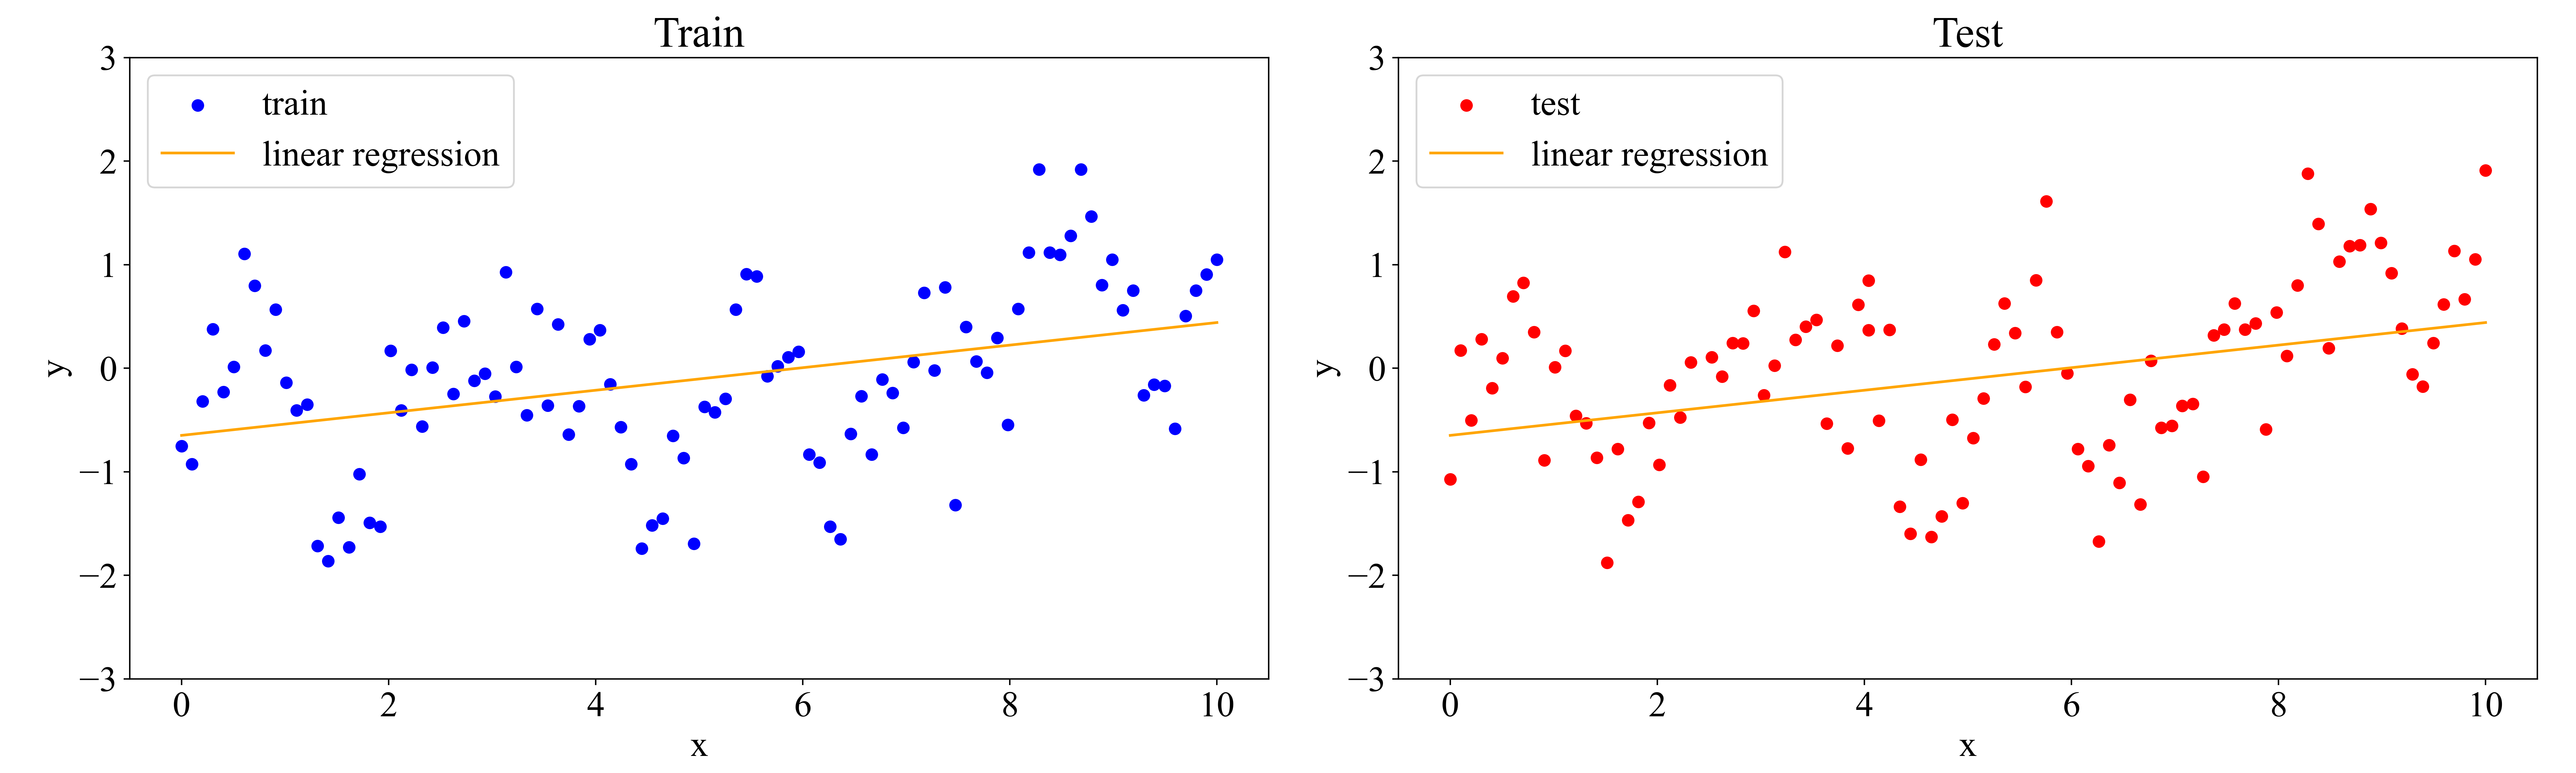
\includegraphics[width=0.8\linewidth]{figure/linear_regression.png}
    \caption{Linear regression fits on training and testing data.}
    \label{fig:linear_regression}
\end{figure}
Illustrated in \Cref{fig:linear_regression}, the linear regression model fails to capture the nonlinear relationship between the input features and the output values,
corresponding to the poor performance in metrics above.

\subsection{Polynomial Regression}
\begin{table}[H]
    \centering
    \caption{Performance of polynomial regression for different degrees.}
    \label{tab:poly_results}
    \begin{tabular}{lcccc}
        \toprule
        Degree & \multicolumn{2}{c}{Training} & \multicolumn{2}{c}{Testing} \\
        \cmidrule(r){2-3} \cmidrule(l){4-5}
        & RMSE & $R^2$ & RMSE & $R^2$ \\
        \midrule
        1 & 0.7832 & 0.1413 & 0.7714 & 0.1329 \\
        2 & 0.7519 & 0.2084 & 0.7312 & 0.2209 \\
        3 & 0.7519 & 0.2086 & 0.7327 & 0.2178 \\
        4 & 0.7456 & 0.2218 & 0.7361 & 0.2104 \\
        5 & 0.7247 & 0.2648 & 0.7177 & 0.2493 \\
        6 & 0.7247 & 0.2648 & 0.7177 & 0.2494 \\
        7 & 0.6820 & 0.3489 & 0.6805 & 0.3252 \\
        8 & 0.6793 & 0.3541 & 0.6797 & 0.3268 \\
        9 & 0.5951 & 0.5043 & 0.6225 & 0.4354 \\
        10 & 0.5914 & 0.5104 & 0.6195 & 0.4408 \\
        11 & $\mathbf{0.5495}$ & $\mathbf{0.5773}$ & $\mathbf{0.5784}$ & $\mathbf{0.5125}$ \\
        12 & 0.5516 & 0.5741 & 0.5865 & 0.4987 \\
        13 & 0.7689 & 0.1723 & 0.7236 & 0.2370 \\
        14 & 0.6524 & 0.4041 & 0.7291 & 0.2253 \\
        \bottomrule
    \end{tabular}
\end{table}
As shown in \Cref{tab:poly_results}, the performance of polynomial regression improves significantly as the degree of the polynomial increases ranging from 1 to 11.
But after degree 11, the performance starts to degrade, which may influenced by extreme values in high degrees.
When the degree equals 1, polynomial regression degenerates to linear regression, which is consistent with the results in \Cref{tab:baseline_results}.
Any polynomial regression with degree higher than 1 in \Cref{tab:poly_results} outperforms the linear regression, due to its ability to capture more complex patterns in the data.
\begin{figure}[H]
    \centering
    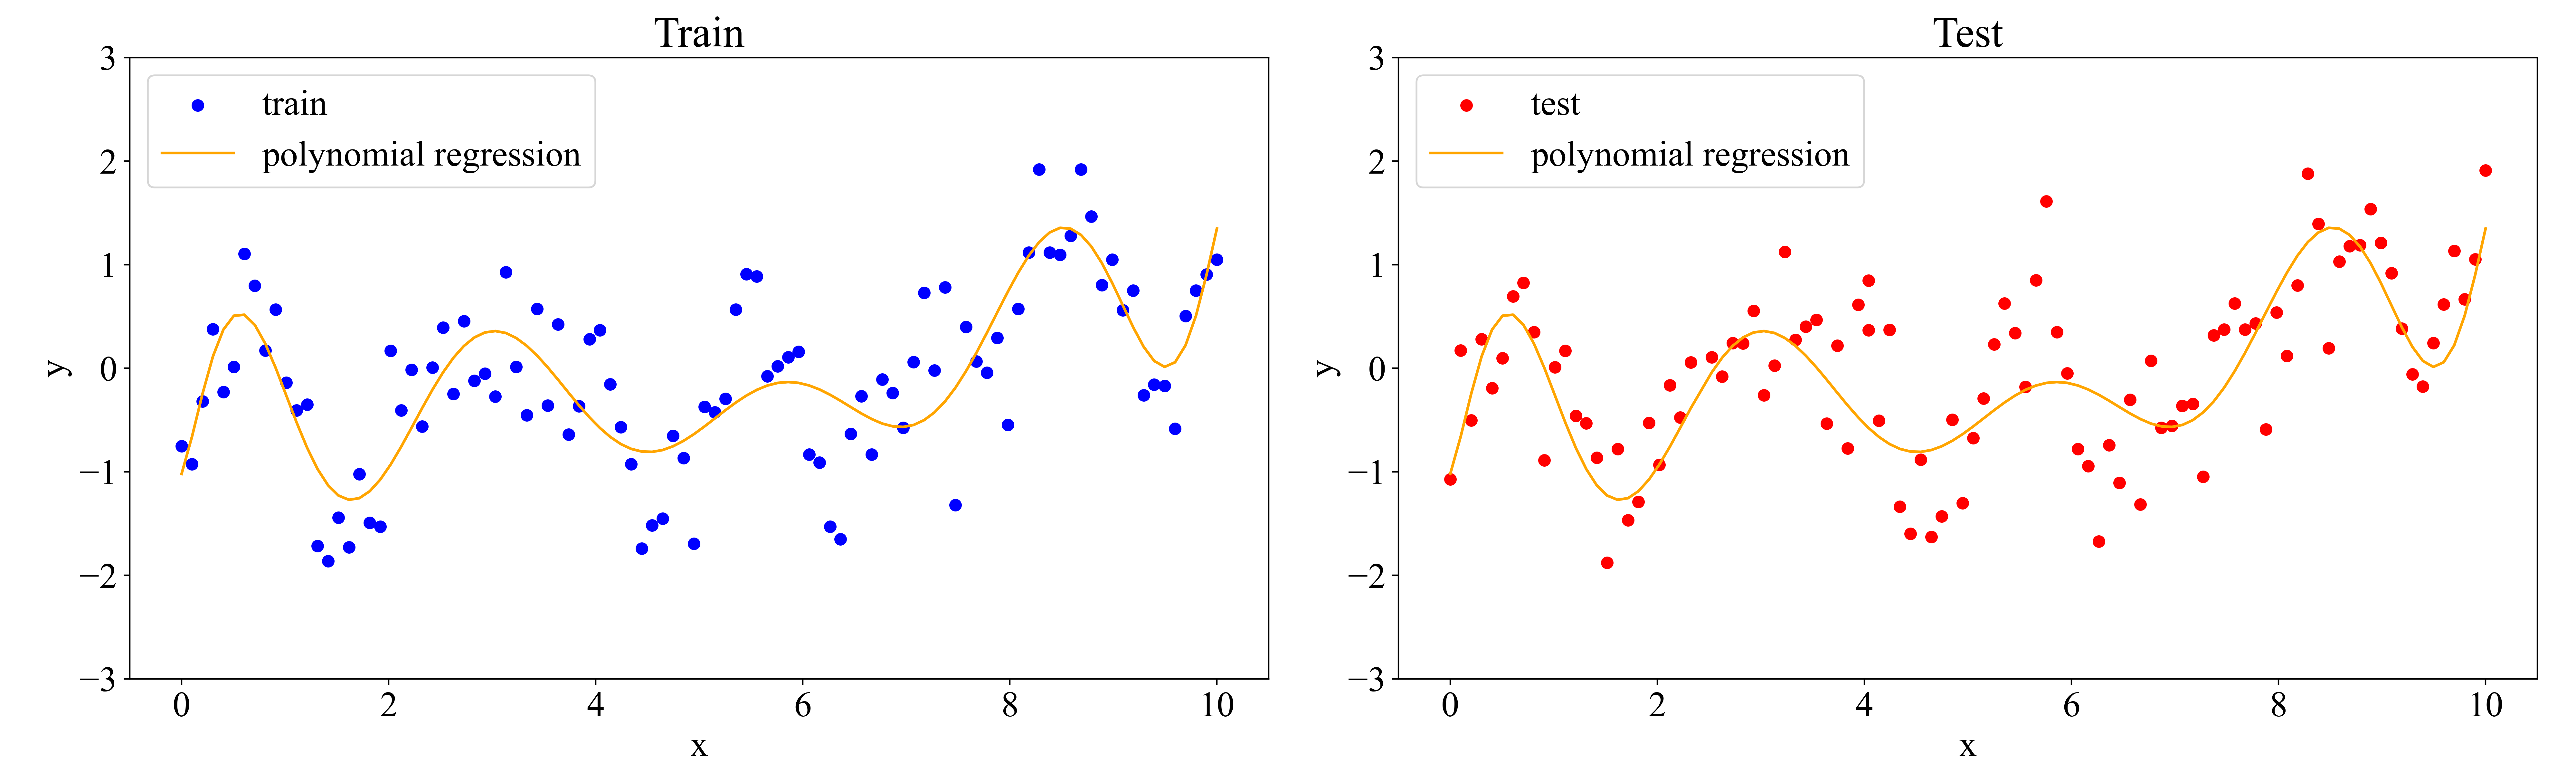
\includegraphics[width=0.8\linewidth]{figure/polynomial_regression.png}
    \caption{Polynomial regression fit with 11th-degree polynomial.}
    \label{fig:polynomial_regression}
\end{figure}
It is important to note that as the degree of the polynomial increases, there is a risk of overfitting.
Demonstrated in \Cref{fig:polynomial_regression}, the 11th-degree polynomial regression model fits the training data the best.


\subsection{Kernel Regression}
\begin{table}[H]
    \centering
    \caption{Performance of kernel regression(using Gaussian kernel) with different bandwidths.}
    \label{tab:kernel_results}
    \begin{tabular}{lcccc}
        \toprule
        Bandwidth & \multicolumn{2}{c}{Training} & \multicolumn{2}{c}{Testing} \\
        \cmidrule(r){2-3} \cmidrule(l){4-5}
        & RMSE & $R^2$ & RMSE & $R^2$ \\
        \midrule
        0.1 & $\mathbf{0.3178}$ & $\mathbf{0.8586}$ & $\mathbf{0.5067}$ & $\mathbf{0.6259}$ \\
        0.25 & 0.4499 & 0.7167 & 0.5092 & 0.6221 \\
        0.5 & 0.6004 & 0.4953 & 0.6037 & 0.4689 \\
        1.0 & 0.7165 & 0.2814 & 0.7030 & 0.2798 \\
        1.5 & 0.7451 & 0.2227 & 0.7326 & 0.2179 \\
        \bottomrule
    \end{tabular}
\end{table}
As shown in \Cref{tab:kernel_results}, the performance of kernel regression is highly sensitive to the choice of bandwidth parameter.
A smaller bandwidth (0.1) leads to a better fit to the training data, resulting in a lower RMSE and higher $R^2$ value.
However, it's test performance is not as good as the training performance, which may indicate some degree of overfitting with bandwidth 0.1.
\begin{figure}[H]
    \centering
    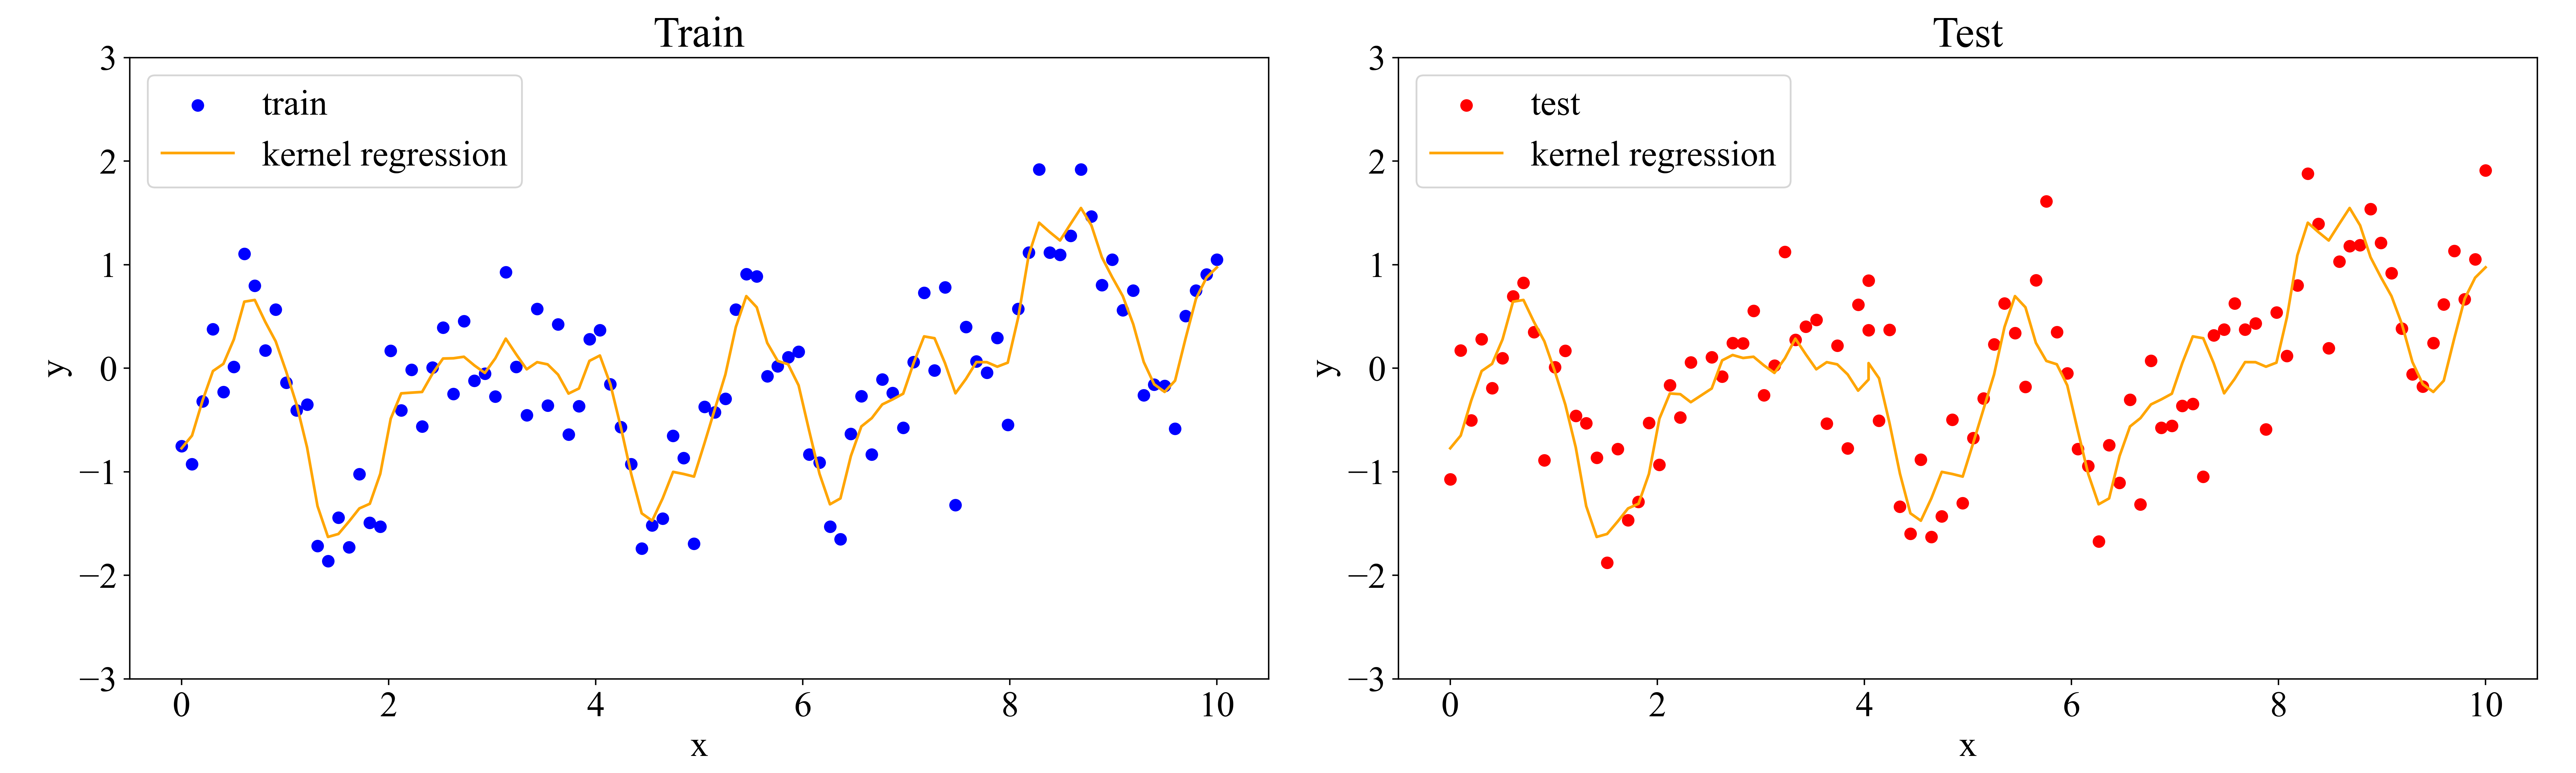
\includegraphics[width=0.8\linewidth]{figure/kernel_regression_0.1.png}
    \caption{Kernel regression fit with bandwidth of 0.1.}
    \label{fig:kernel_regression_0.1}
\end{figure}
\begin{figure}[H]
    \centering
    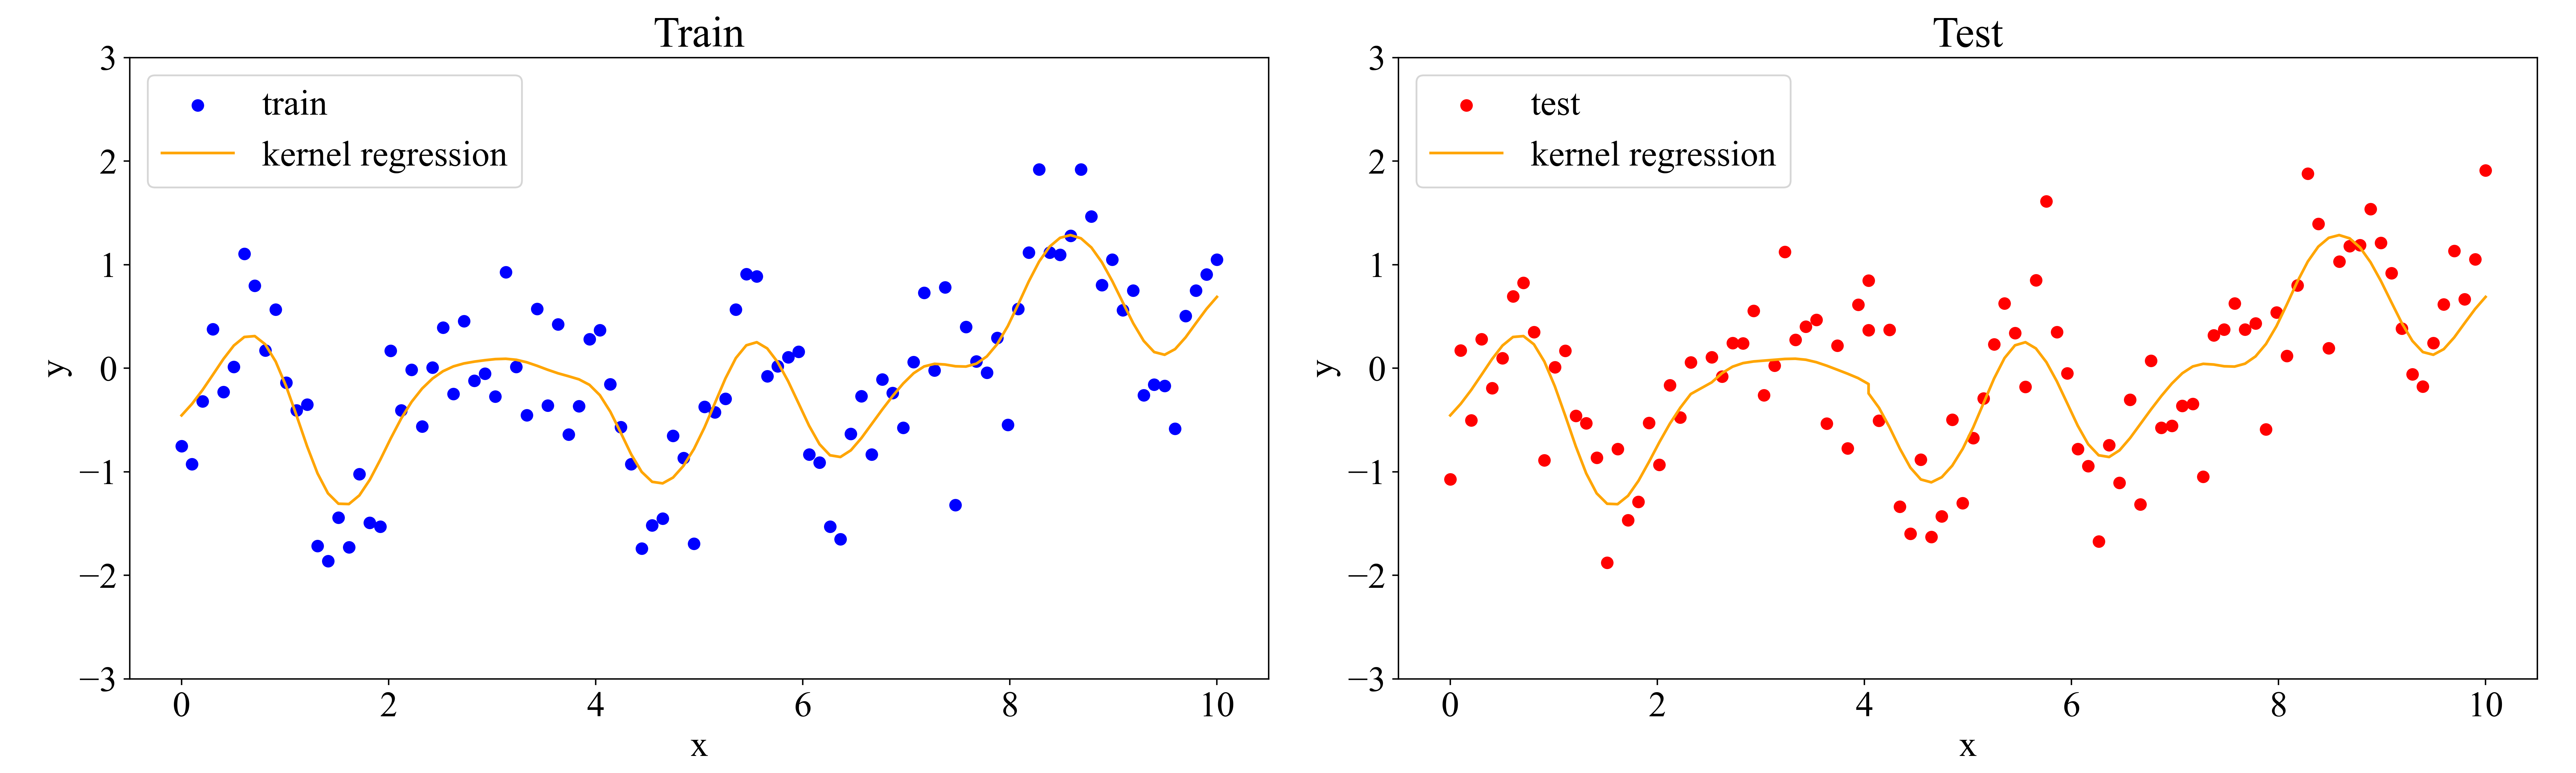
\includegraphics[width=0.8\linewidth]{figure/kernel_regression_0.25.png}
    \caption{Kernel regression fit with bandwidth of 0.25.}
    \label{fig:kernel_regression_0.25}
\end{figure}
\begin{figure}[H]
    \centering
    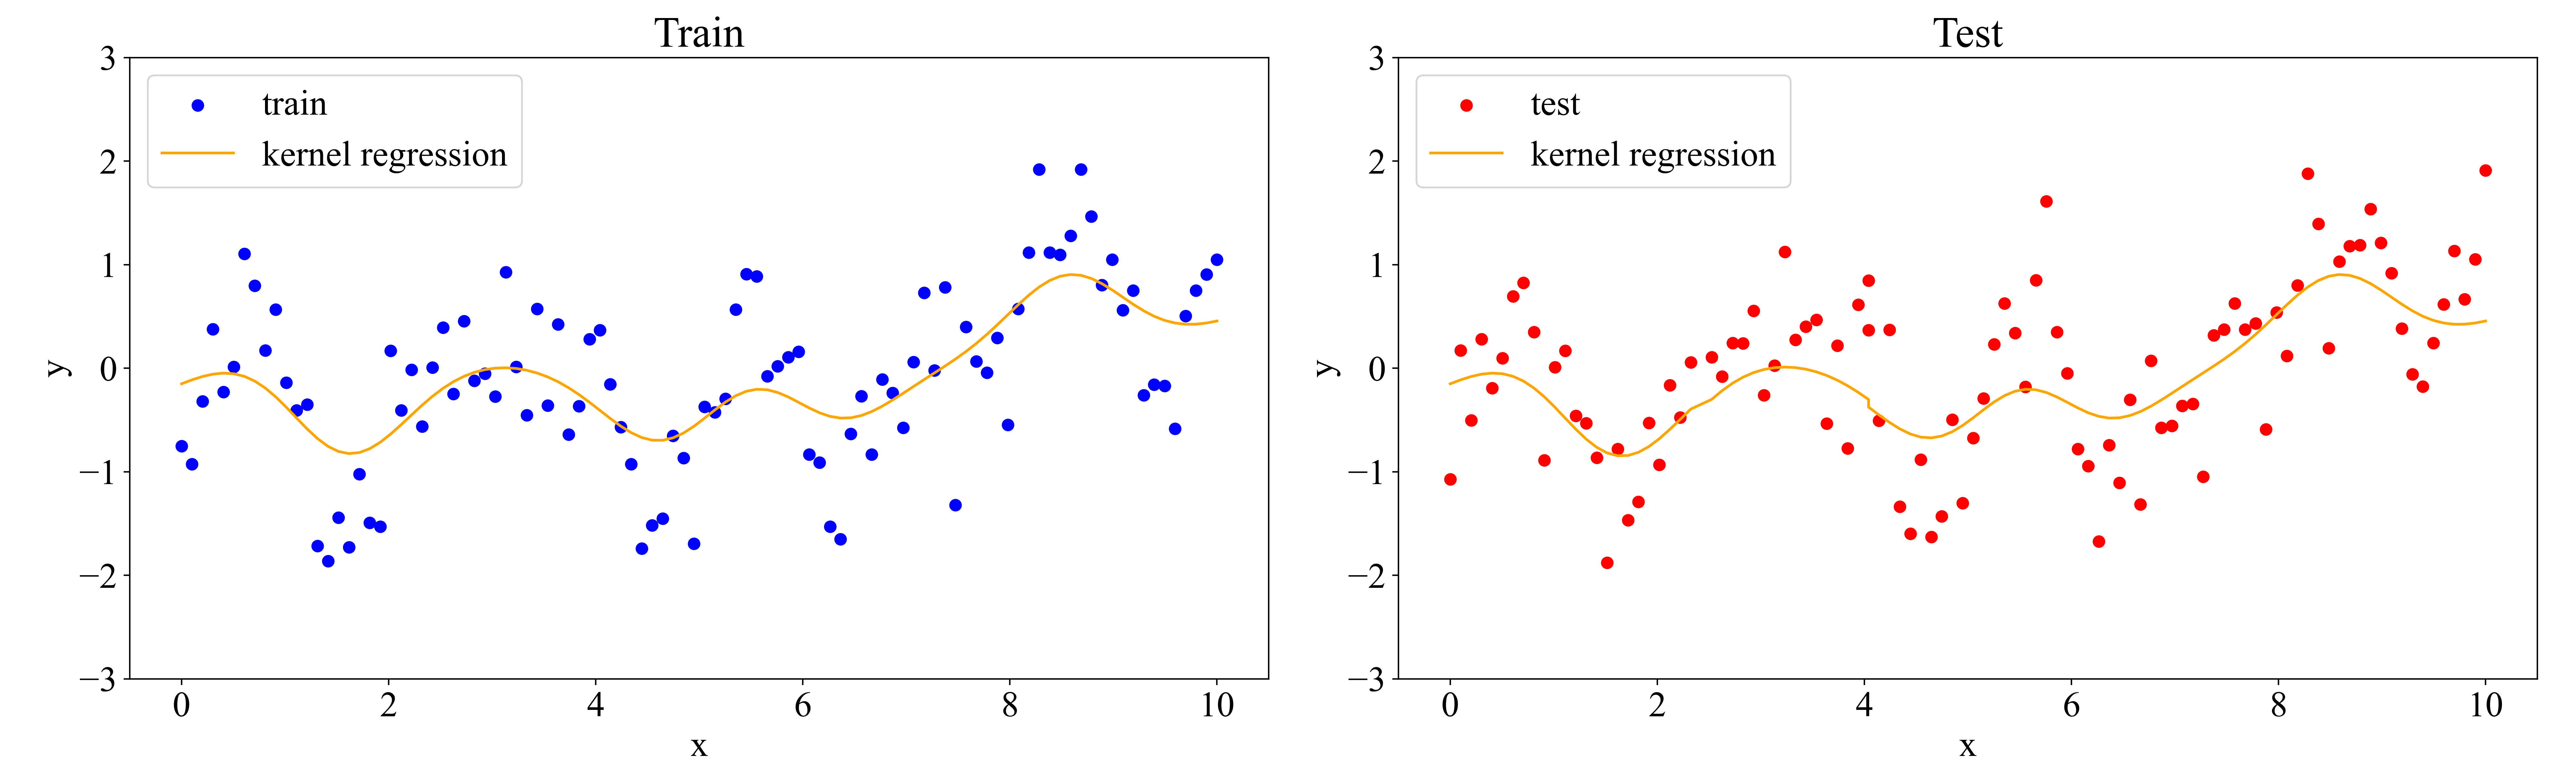
\includegraphics[width=0.8\linewidth]{figure/kernel_regression_0.5.png}
    \caption{Kernel regression fit with bandwidth of 0.5.}
    \label{fig:kernel_regression_0.5}
\end{figure}
\begin{figure}[H]
    \centering
    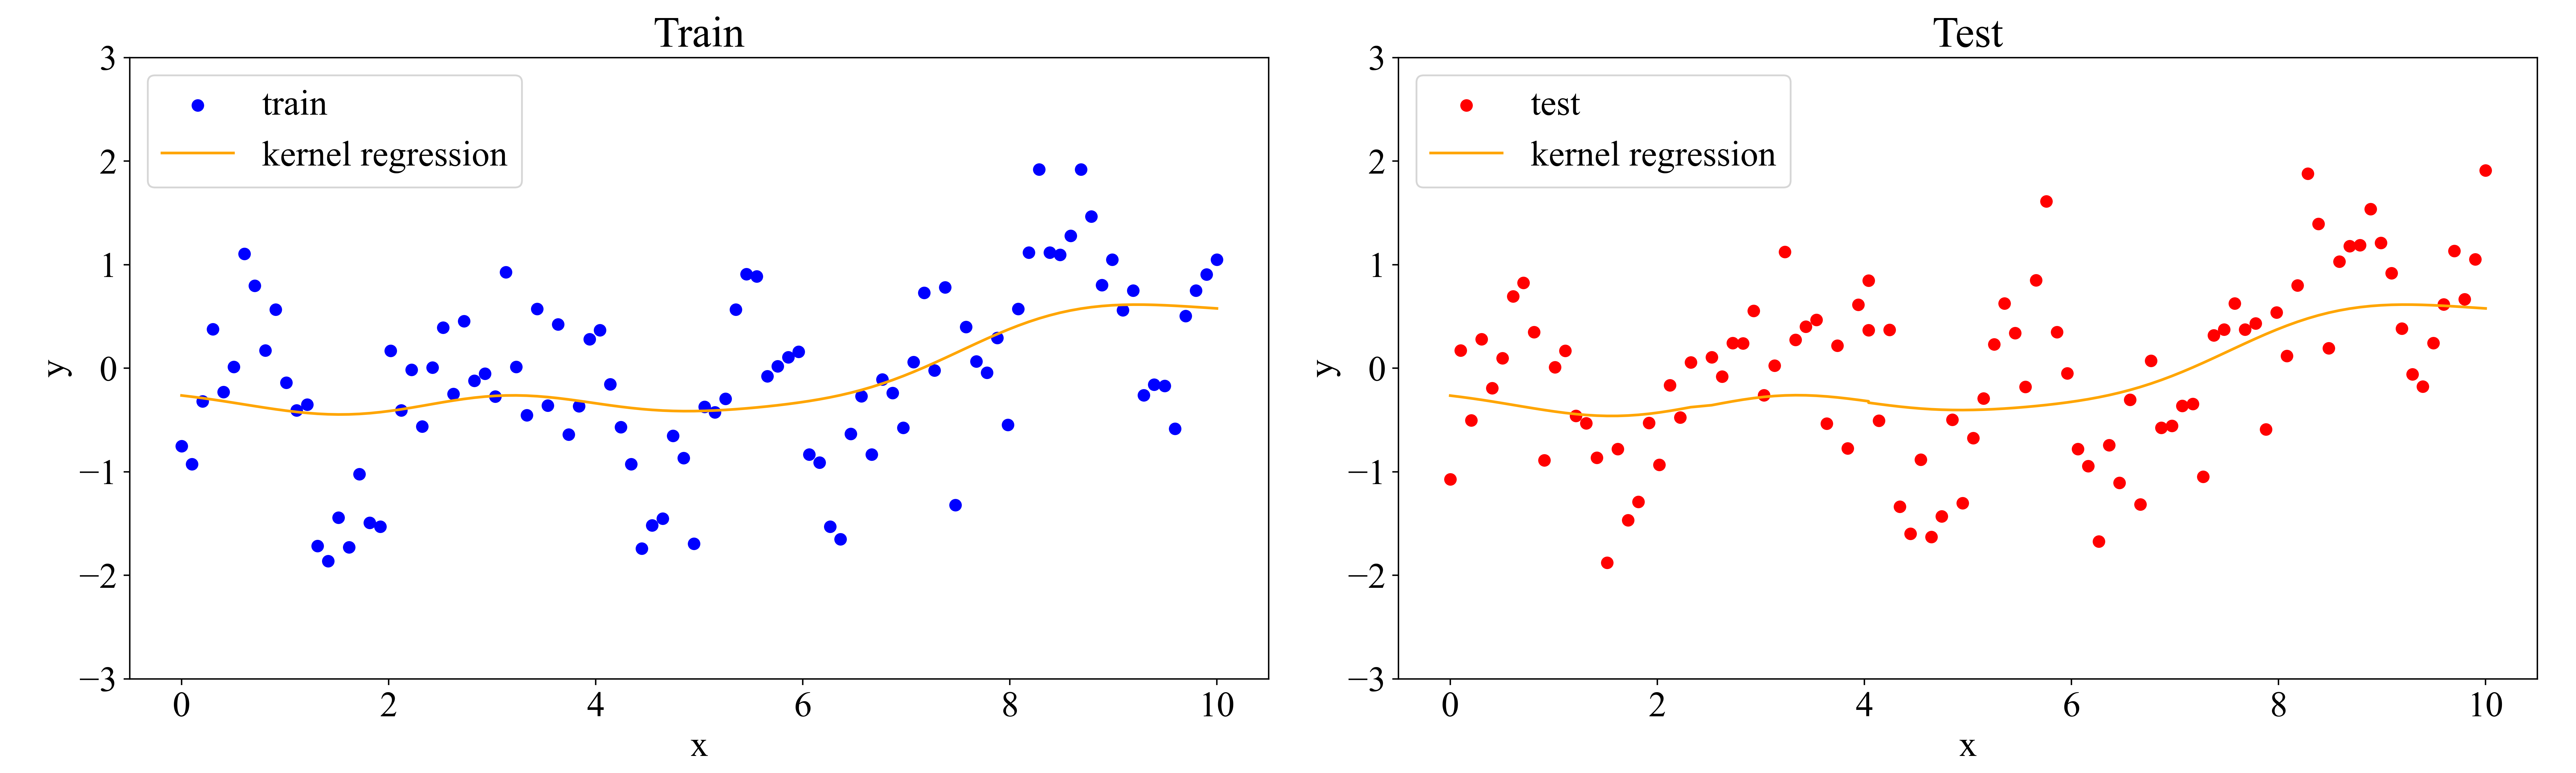
\includegraphics[width=0.8\linewidth]{figure/kernel_regression_1.0.png}
    \caption{Kernel regression fit with bandwidth of 1.0.}
    \label{fig:kernel_regression_1.0}
\end{figure}
As the bandwidth increases, the model becomes smoother and less sensitive to data, which can lead to underfitting.
In this case, the bandwidth of 0.25 and 0.1 perform nearly the same.


\section{Conclusions}
\label{sec:conclusions}
In this paper, we have explored the performance of different regression models and optimization algorithms on a given dataset.
We found that linear regression, regardless of the optimization algorithm used, did not fit the data well due to the nonlinear relationship between the input features and the output values.
Besides, different optimization algorithms performed similarly but gradient descent may require careful tuning hyperparameters and cost much more time and computational resources.
Polynomial regression with an appropriate degree provided a better fit to the data, but there is a risk of overfitting as the degree increases.
Kernel regression showed the best results with RMSE of 0.5067 and $R^2$ of 0.6259 for test data, but its performance is highly sensitive to the choice of bandwidth parameter.
Overall, the choice of model and optimization algorithm should be guided by the characteristics of the data and the underlying relationship between the variables.

\printbibliography

% \begin{appendices}

% \section{MATLAB Functions}
% Add your important MATLAB functions here with a brief implementation explanation. This is how to make an \textbf{unordered} list:
% \begin{itemize}
%     \item \texttt{y = linspace(x1,x2,n)} returns a row vector of \texttt{n} evenly spaced points between \texttt{x1} and \texttt{x2}. 
%     \item \texttt{[X,Y] = meshgrid(x,y)} returns 2-D grid coordinates based on the coordinates contained in the vectors \texttt{x} and \texttt{y}. \text{X} is a matrix where each row is a copy of \texttt{x}, and \texttt{Y} is a matrix where each column is a copy of \texttt{y}. The grid represented by the coordinates \texttt{X} and \texttt{Y} has \texttt{length(y)} rows and \texttt{length(x)} columns.  
% \end{itemize}

% \end{appendices}

\end{document}
